\newpage
\section{Experiments and Evaluation}

\subsection{Evaluation of the detection node.}

For the whole system to succeed, it is extremely important that the image detection algorithm is robust and with high accuracy rates. To evaluate its performance, the detector was tested on a video sequence such as the one shown in figure \ref{fig:feature_extraction}, achieving almost 100\% of accuracy detecting the ball in working conditions. However, we discovered that shadows can make the detector unreliable. Furthermore, having multiple red objects in the scene will result in a fail.

\subsection{Evaluation of the triangulation node.}

The triangulation node was evaluated with a test program which received the messages and transform it to robot base coordinates. In that way, moving the obstacle along the XYZ axes of the robot's base frame, it could be checked on the program if the X, Y, and Z coordinates were correctly assigned.

\subsection{Evaluation of the Kalman filter}
Three test are designed in order to evaluate the functionality and performance of the 3D Kalman Filter. As the objective is to track the ball.

We elaborated a first test based on motion tracking, where the ball is missing for a period of time and the statistical algorithm is able to predict the position of the ball . 
The second test is designed to determine which values for the process and measurement covariances matrices are needed for a good performance of the filter. Lastly, a third test that will prove how the Kalman Filter behaves with a miss recognition of the ball.
\newpage
\subsubsection{Test 1: Motion tracking}
The Kalman filter state considers the position, velocity, and acceleration of the ball. This allows the filter to learn the motion of the ball. So if we expect to loss the ball in a trajectory, the statistical algorithm will predict the next states of the ball based on the motion of the lasts measurements it got. In a practical point of view, the Kalman filter is able to remember the linear motion that the ball had, so if we are moving the ball linearly it will consider that motion and predict based on that. Non-linearities when the ball is missing would be not considered by the algorithm.

The test is quite simple, first of all we put the ball in one corner of the camera range and we start moving smoothly the ball by using a stick. The movement is a linear movement, but suddenly the ball passes behind the robot without being in camera range. It can be observed in the red line of the fig. \ref{fig:kf_motion} that the measurements are gone in that moment. However, the Kalman filter is able to predict the linear trajectory and in the end when the ball is in the camera range the Kalman Filter corrects its states.
%\vspace{3 pt}
\begin{figure}[ht!]
    \centering
    \captionsetup{justification=centering,margin=1cm}
    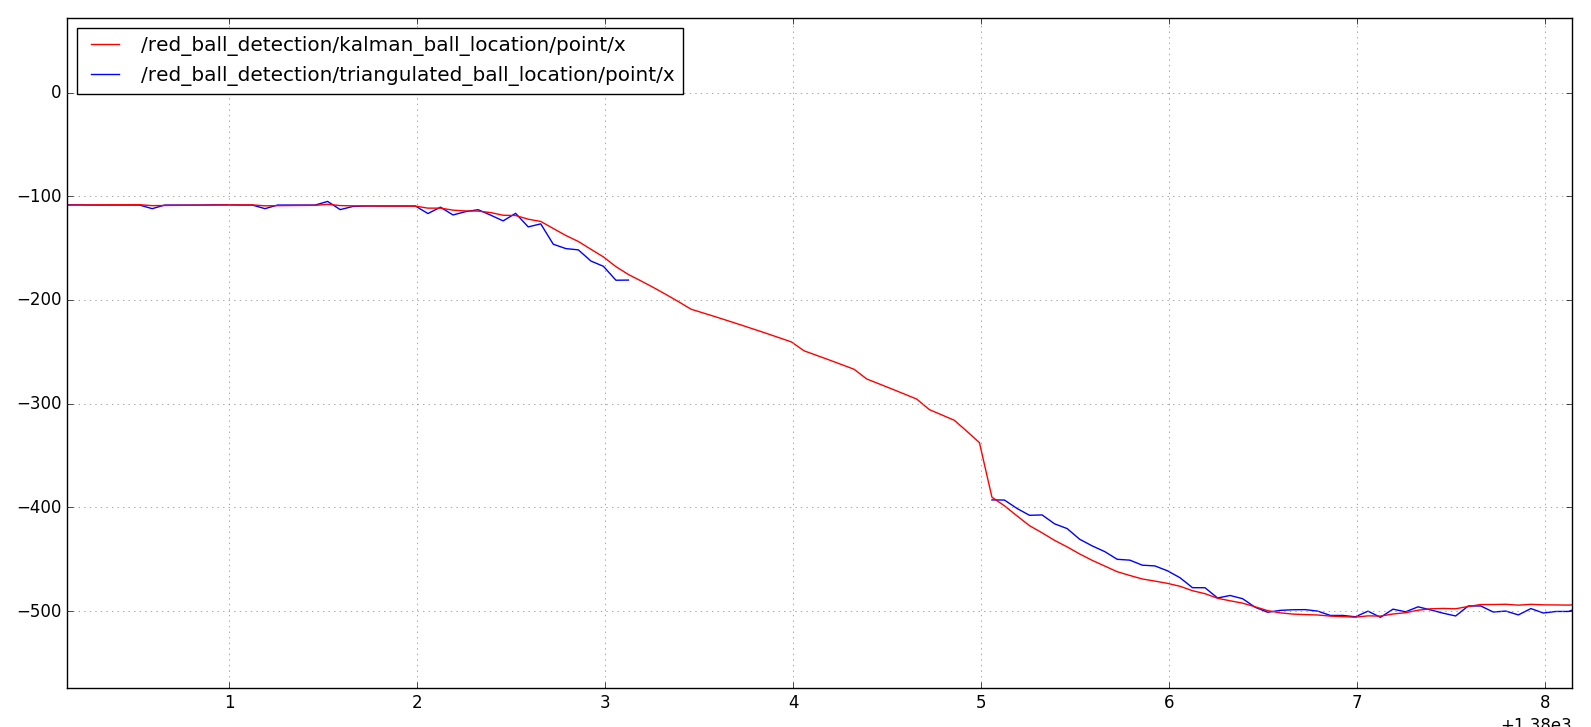
\includegraphics[scale = 0.30]{Images/kf/motion_tracking.png}
    \caption[]{Kalman Filter motion tracking.}
    \label{fig:kf_motion}
\end{figure}%

% PLOT!
% lets make a test moving the ball continously with a low-noise R and Q to see what happens, it will show a sinousoid??? KF is linear!! :S
\newpage
\subsubsection{Test 2: Uncertainty in Kalman Filter}

The second test consist in moving the ball continuously in 'x' axis for different noise levels in measurement and process covariances matrices. The purpose is to see how the filter adapts itself in the motion described. Moreover, it is expected to determine which values are suitable for our application. In fact, we want to determine the motion that the \textit{Kalman Filter} should track. Moreover, we need to know how fast is the ball suppose to move. Faster motions than expected should be filtered.

The motion that defines the limit where the filter should act is found empirically. The ball is moved from two states in 'x' direction with the motion we should remove. In fig. \ref{fig:kf_uncertainty} left side is noticeable how the Kalman Filter adapts to the motion completely. The motion applied to the ball is quite fast, so a miss detection of the ball in a remote place on the workcell would lead to a bad tracking of the ball. In the right side of the image is observed that the output of the Kalman Filter is a bit smooth compared with the previous image. In this case, the statistical algorithm with high-level noise is more robust to out-layers rather than the previous performance of the filter.
\begin{figure}[ht!]
\centering
\captionsetup{justification=centering,margin=1cm}
\resizebox{\textwidth}{!}{\begin{tabular}{cc}
%\hline
\subf{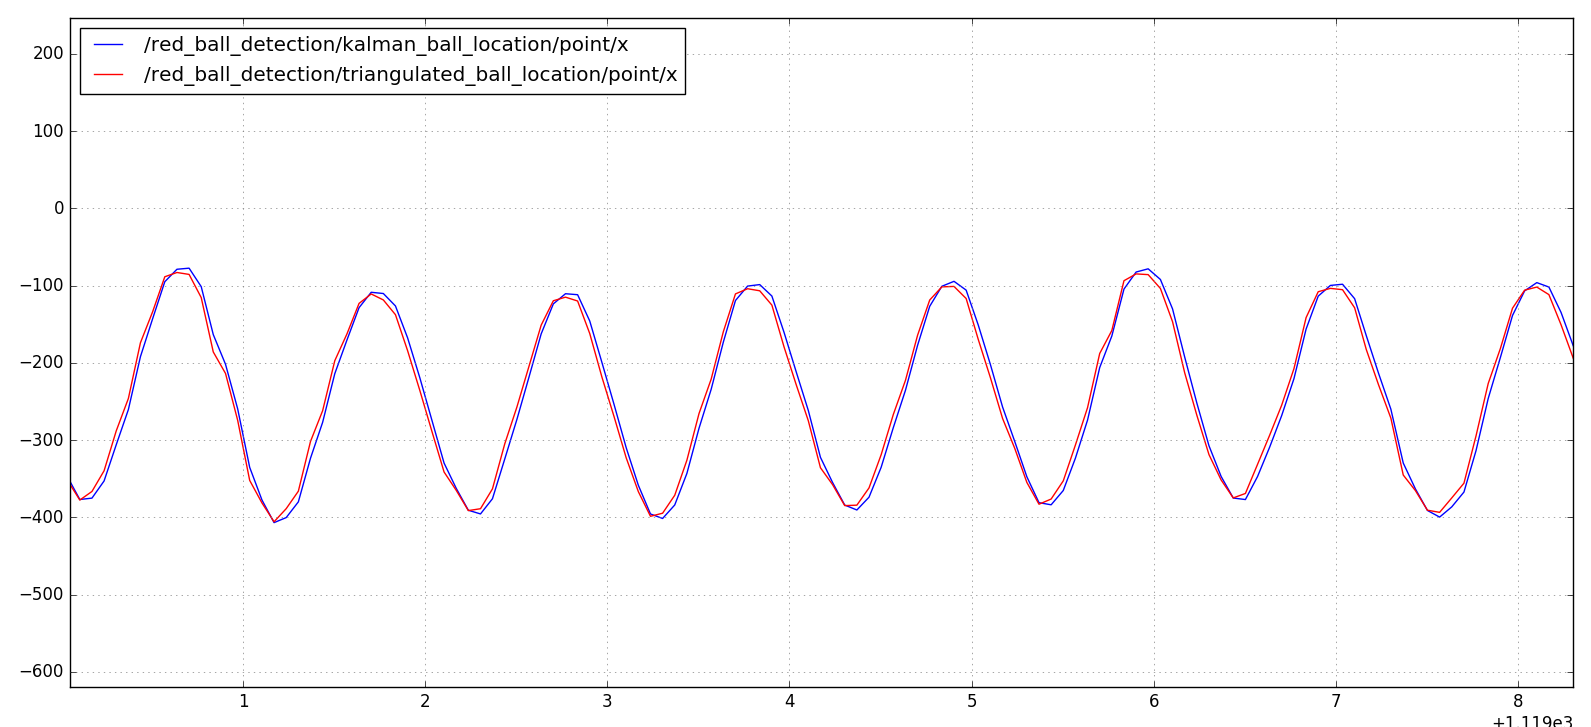
\includegraphics[width=60mm,height=60mm]{Images/kf/noise_0p1.png}}
     {Kalman filter R and Q with 0.1}
&
\subf{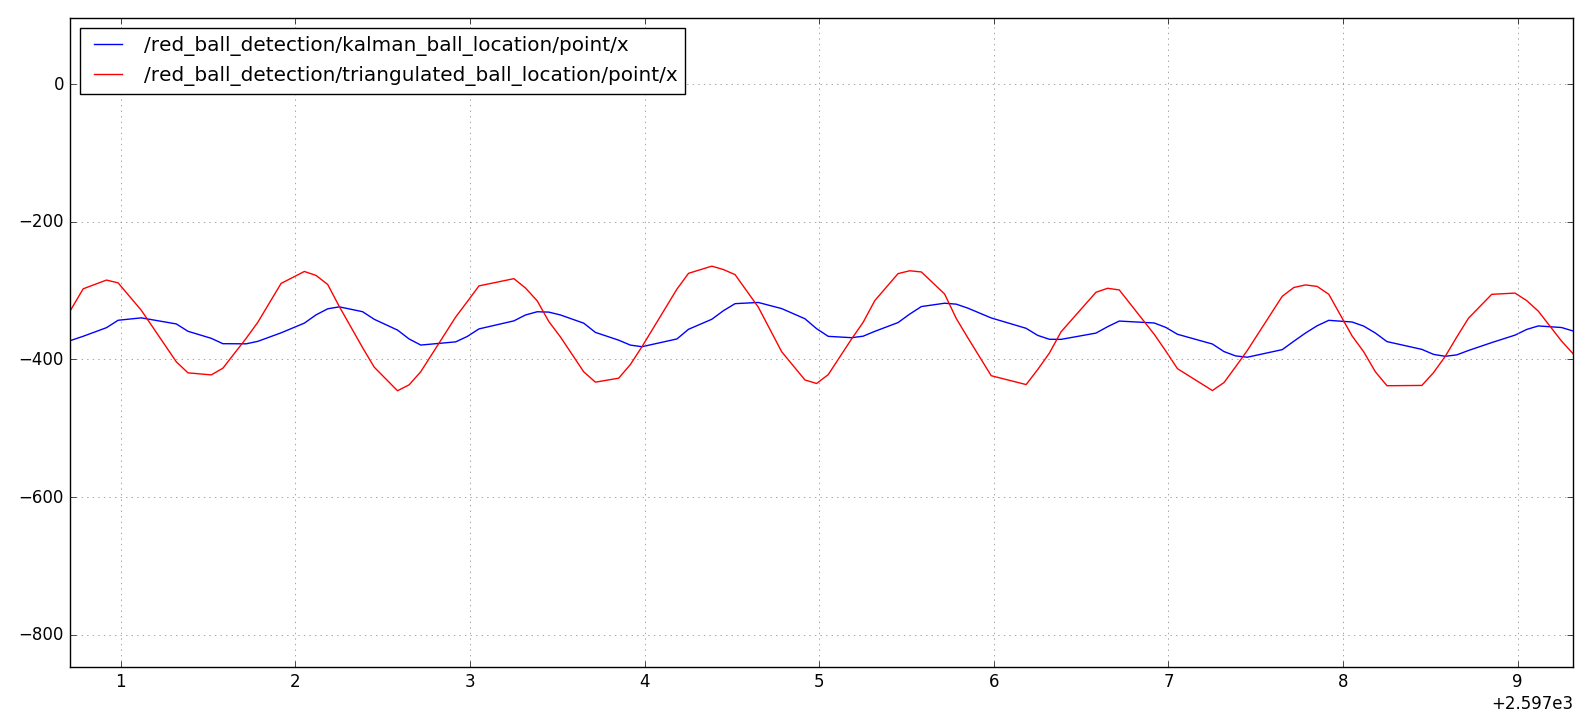
\includegraphics[width=60mm,height=60mm]{Images/kf/noise_150.png}}
     {Kalman filter R: 150 and Q: 0.1}
%\hline
\end{tabular}}
\caption{Uncertainty in measurement.}
\label{fig:kf_uncertainty}
\end{figure}  
   
\newpage
\subsubsection{Test 3: Miss recognition}

The third test consist to reproduce a miss recognition of the ball's position. For doing that, we grab the ball with our hand covered by black clothes and do a really fast movement of the ball in axis 'x'. 

Using the same levels of noise as before. It is found something interesting, the filter with low-noise levels is almost adapted by one measurement. The differential position is about 30 cm, which makes the Kalman Filter a really fast approach to a motion that moves 30 cm per measurement. However, this performance does not fit very well to our system specifications. A movement with those characteristics should be filtered. In the right-side of the figure and with a high level noise in covariances matrices the filter performs really well in our own specifications because it does not adapt that good to the motion specified, but in fact it starts to do it. So we expect to adapt completely in 3-4 measurements. 

In this case, the main key point is to define the expectation of a miss recognition. For this project it is considered around 3-4 measurements a valid move of the ball, mainly because, the motion is not clearly defined. The ball is moved with a stick which makes the system quite impredecible and the Kalman Filter needs to track the ball for those movements. 
% In order to reduce the complexity the movement of the ball could be linear defined so the ball is able to track it. Or an extended Kalman filter or unscented Kalman filter can be applied
\begin{figure}[ht!]
\centering
\captionsetup{justification=centering,margin=1cm}
\resizebox{\textwidth}{!}{\begin{tabular}{cc}
%\hline
\subf{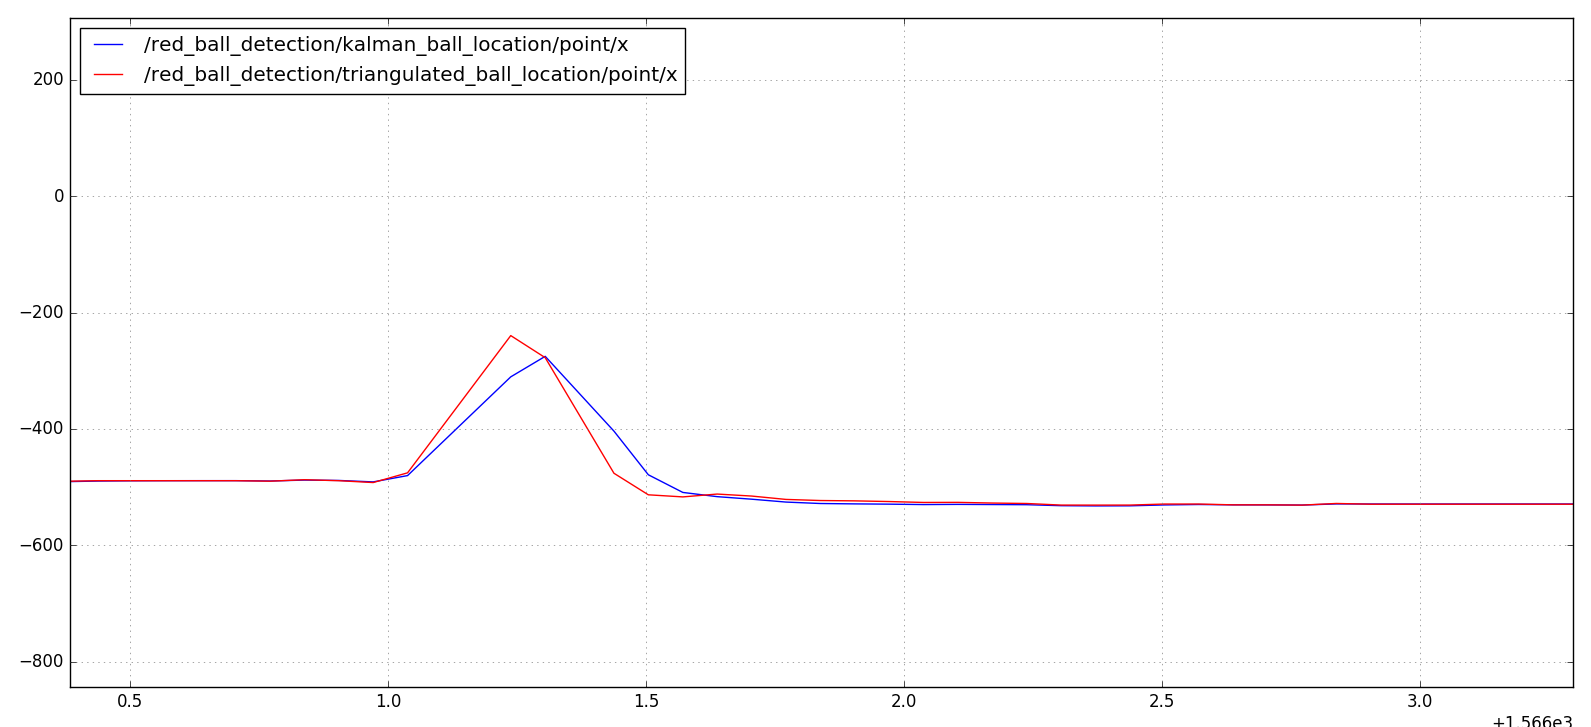
\includegraphics[width=60mm,height=60mm]{Images/kf/misrecognition_noise0p1.png}}
     {Kalman filter low-noise levels}
&
\subf{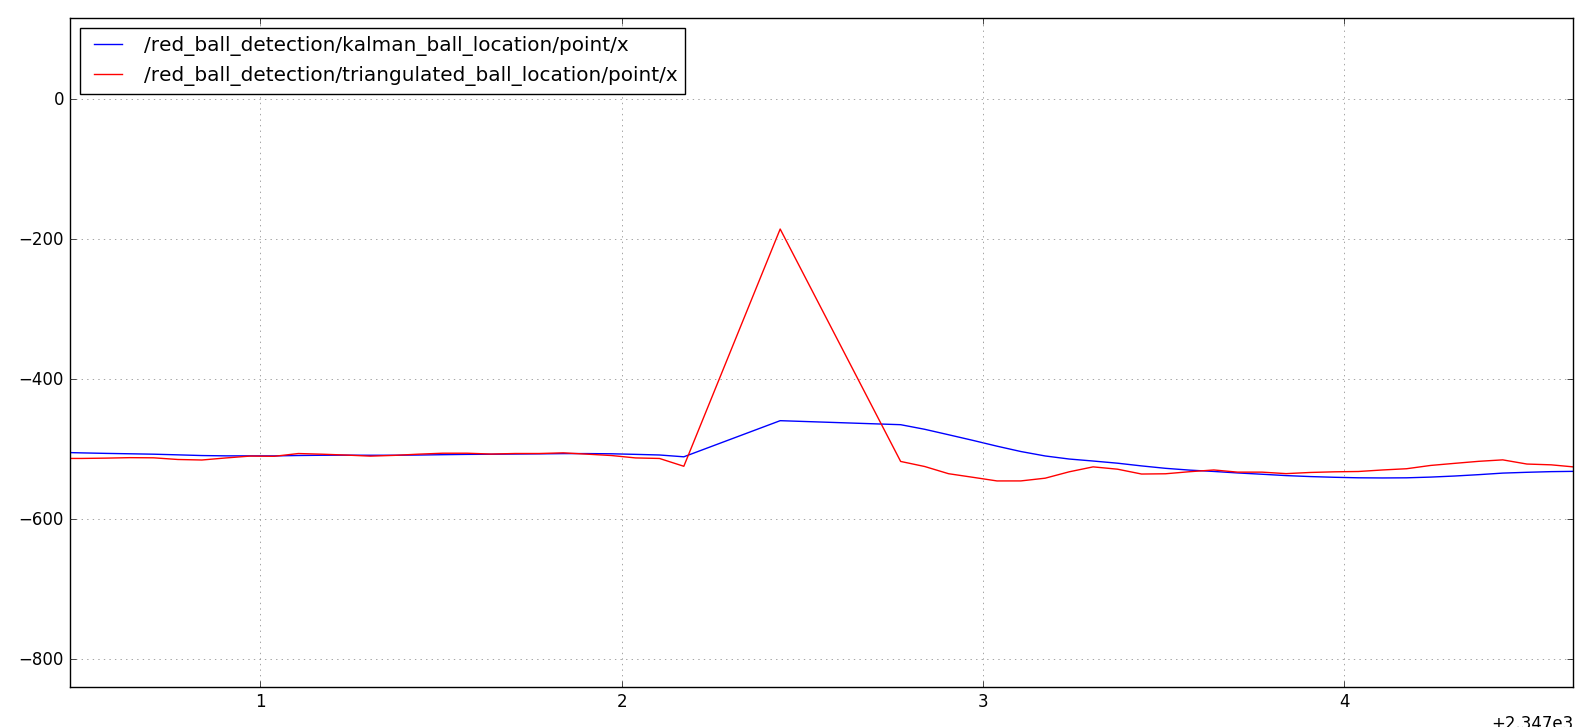
\includegraphics[width=60mm,height=60mm]{Images/kf/misrecognition_noise150.png}}
     {Kalman filter high noise}
%\hline
\end{tabular}}
\caption{Miss recognition in measurement.}
\label{fig:kf_uncertainty}
\end{figure}  
\section{Results}

In this sections is exposed the performance of the algorithms which this project focuses on: The RRT* planner for the robotics side and the Kalman filter for the vision side.

In order to evaluate the Kalman Filter: the computation time, error response for different noise levels. The execution time of the statistical algorithm is \textbf{51 $\mu$s} which makes sense due the fact that this algorithm is used for applications where the computational time is required to be low.

In order to see how the different noise levels in the process and measurement covariance matrices affects the performance of the Kalman filter. It is decided to choose between high and low values and switch the combinations to see how is the error in motion tracking. The empirical tests has been done in static and dynamic environments.
\begin{figure}[ht!]
\begin{subfigure}{.5\textwidth}
  \centering
  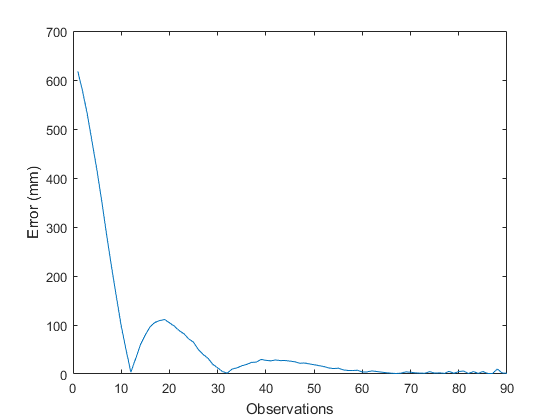
\includegraphics[width=.8\linewidth]{Images/kalman_plots/static_1.png}
  \caption{Static-1: Q = 0.01 and R = 1}
  \label{fig:sfig1}
\end{subfigure}
\begin{subfigure}{.5\textwidth}
  \centering
  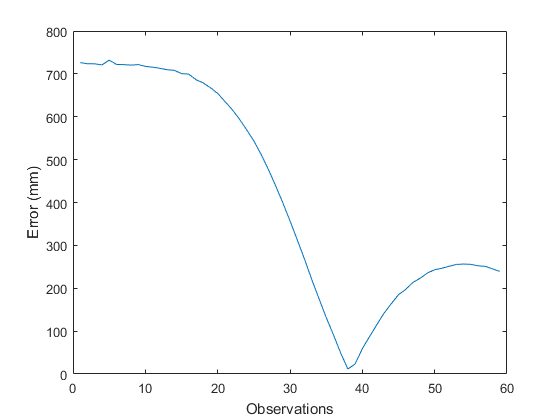
\includegraphics[width=.8\linewidth]{Images/kalman_plots/static_2.png}
  \caption{Static-2: Q = 0.01 and R = 100}
  \label{fig:sfig2}
\end{subfigure}
\begin{subfigure}{.5\textwidth}
  \centering
  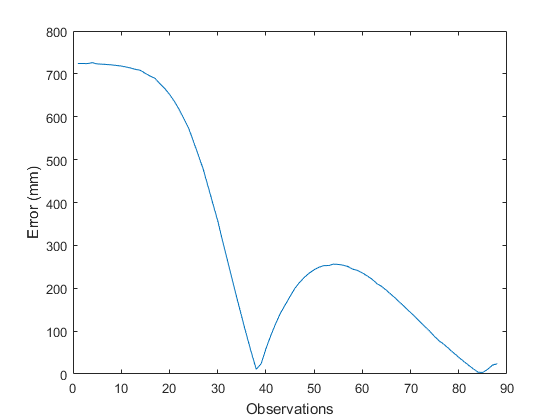
\includegraphics[width=.8\linewidth]{Images/kalman_plots/static_3.png}
  \caption{Static-3: Q = 200 and R = 0.1}
  \label{fig:sfig3}
\end{subfigure}
\begin{subfigure}{.5\textwidth}
  \centering
  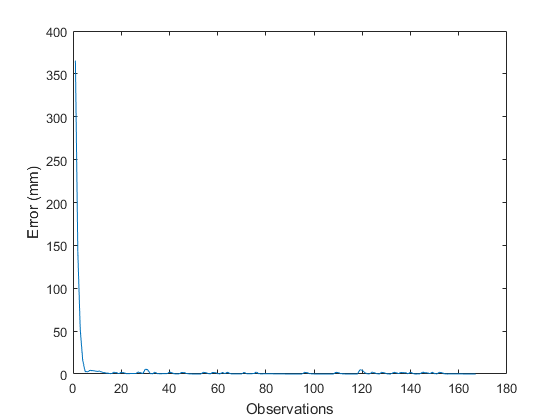
\includegraphics[width=.8\linewidth]{Images/kalman_plots/static_4.png}
  \caption{Static-4: Q = 300 and R = 300}
  \label{fig:sfig4}
\end{subfigure}
\caption{Error plots of the Kalman filter and measurement in static.}
\label{fig:static_kalman}
\end{figure}

To check the error of the Kalman Filter in dynamic environment see section \ref{sec:annex}.
\newpage
To evaluate the anytime dynamic path planner performance, we investigated run-time of the collision checker algorithm against the resolution. We used pruned paths from the initial to the end configuration each time and performed collision checking 20, 50 and 500 configurations between each node.

50 measurements where taken at each level and the averages are shown in Table \ref{tab:coll}.
\begin{table}[ht!
]
\centering
\label{plan:accuracy_table}
    \begin{tabular}{|c|c|}
    \hline
    Nº Nodes & Time(s))  \\ \hline
      108       &  0.195     \\ \hline
      243      & 0.21      \\ \hline
        2561      &  0.38       \\ \hline
    \end{tabular}
    \caption[]{\textit{ Collision performance.}}
    \label{tab:coll}
\end{table}

We measured the runtime of the planner from the initial configuration to the final one. We investigated the number of nodes generated and the resulting path after pruning. We took 50 measurements at each level of the extend parameters and we plot the averages in Table \ref{tab:plan}

\begin{table}[H]
\centering
\label{plan:accuracy_table}
    \begin{tabular}{|c|c|c|c|}
    \hline
    Extend ($\epsilon$)  & Nº Nodes & Nº Nodes (opt.) & Planner time(s)  \\ \hline
    0.05          &  193  & 6 &  0.47   \\ \hline
    0.2              &  51 & 5 & 0.070    \\ \hline
    0.5          & 24 & 4 & 0.026   \\ \hline
    2          &  6 & 3 & 0.007      \\ \hline

    \end{tabular}
    \caption[]{\textit{RRT*} performance.}
    \label{tab:plan}
\end{table}

